\documentclass[12pt]{article}\usepackage[]{graphicx}\usepackage[]{color}
%% maxwidth is the original width if it is less than linewidth
%% otherwise use linewidth (to make sure the graphics do not exceed the margin)
\makeatletter
\def\maxwidth{ %
  \ifdim\Gin@nat@width>\linewidth
    \linewidth
  \else
    \Gin@nat@width
  \fi
}
\makeatother

\definecolor{fgcolor}{rgb}{0.345, 0.345, 0.345}
\newcommand{\hlnum}[1]{\textcolor[rgb]{0.686,0.059,0.569}{#1}}%
\newcommand{\hlstr}[1]{\textcolor[rgb]{0.192,0.494,0.8}{#1}}%
\newcommand{\hlcom}[1]{\textcolor[rgb]{0.678,0.584,0.686}{\textit{#1}}}%
\newcommand{\hlopt}[1]{\textcolor[rgb]{0,0,0}{#1}}%
\newcommand{\hlstd}[1]{\textcolor[rgb]{0.345,0.345,0.345}{#1}}%
\newcommand{\hlkwa}[1]{\textcolor[rgb]{0.161,0.373,0.58}{\textbf{#1}}}%
\newcommand{\hlkwb}[1]{\textcolor[rgb]{0.69,0.353,0.396}{#1}}%
\newcommand{\hlkwc}[1]{\textcolor[rgb]{0.333,0.667,0.333}{#1}}%
\newcommand{\hlkwd}[1]{\textcolor[rgb]{0.737,0.353,0.396}{\textbf{#1}}}%

\usepackage{framed}
\makeatletter
\newenvironment{kframe}{%
 \def\at@end@of@kframe{}%
 \ifinner\ifhmode%
  \def\at@end@of@kframe{\end{minipage}}%
  \begin{minipage}{\columnwidth}%
 \fi\fi%
 \def\FrameCommand##1{\hskip\@totalleftmargin \hskip-\fboxsep
 \colorbox{shadecolor}{##1}\hskip-\fboxsep
     % There is no \\@totalrightmargin, so:
     \hskip-\linewidth \hskip-\@totalleftmargin \hskip\columnwidth}%
 \MakeFramed {\advance\hsize-\width
   \@totalleftmargin\z@ \linewidth\hsize
   \@setminipage}}%
 {\par\unskip\endMakeFramed%
 \at@end@of@kframe}
\makeatother

\definecolor{shadecolor}{rgb}{.97, .97, .97}
\definecolor{messagecolor}{rgb}{0, 0, 0}
\definecolor{warningcolor}{rgb}{1, 0, 1}
\definecolor{errorcolor}{rgb}{1, 0, 0}
\newenvironment{knitrout}{}{} % an empty environment to be redefined in TeX

\usepackage{alltt}
\usepackage[top=1in, bottom= 1in, left= 1in, right= 1in]{geometry}
\usepackage[USenglish]{babel} % set the language; greek allows \textgreek{\euro}
\usepackage{multirow} % For tables
\usepackage{graphicx, subfigure} % For graphics
\usepackage{fancyhdr} % Produces fancy headers
\usepackage{setspace} % allows for vsape
\usepackage{natbib} % package to organize literature --> google it!
\usepackage{verbatim} % For including R-code
\usepackage{booktabs} % nicer tables
\usepackage{alltt} % verbatim + highlighting
\usepackage{amsmath} %boldsymbols
\usepackage{lscape} %Querformat
\usepackage{dcolumn} % align at decimal mark
\usepackage{floatrow} % description paragraphs below figures and tables
\usepackage{enumerate} % alter enumerate items (i,ii,iii etc)
\usepackage[colorlinks=true,citecolor=blue,urlcolor=blue]{hyperref}
\setlength{\headheight}{15pt}
% http://en.wikibooks.org/wiki/LaTeX/Page_Layout for additional info
\IfFileExists{upquote.sty}{\usepackage{upquote}}{}

\begin{document}
\begin{center}
  {\Large \textbf{Simulating Efficiency of Voting Rules Depending on Assumptions about Individual Utilities}}
\end{center}

\begin{itemize}
\item For each scenario, I simulated 5000 voters in 200 elections. Each scenario differs with regard to the underlying (distributional) assumptions of individual utilities and candidate positions.
\end{itemize}




\subsection*{First Set of Simulations}
\subsubsection*{Scenario 1a: Independent Uniform Utilities for two Alternatives}

\begin{align*}
U_a,U_b \sim \mathcal{U}(0,1)
\end{align*}

\begin{knitrout}
\definecolor{shadecolor}{rgb}{0.969, 0.969, 0.969}\color{fgcolor}
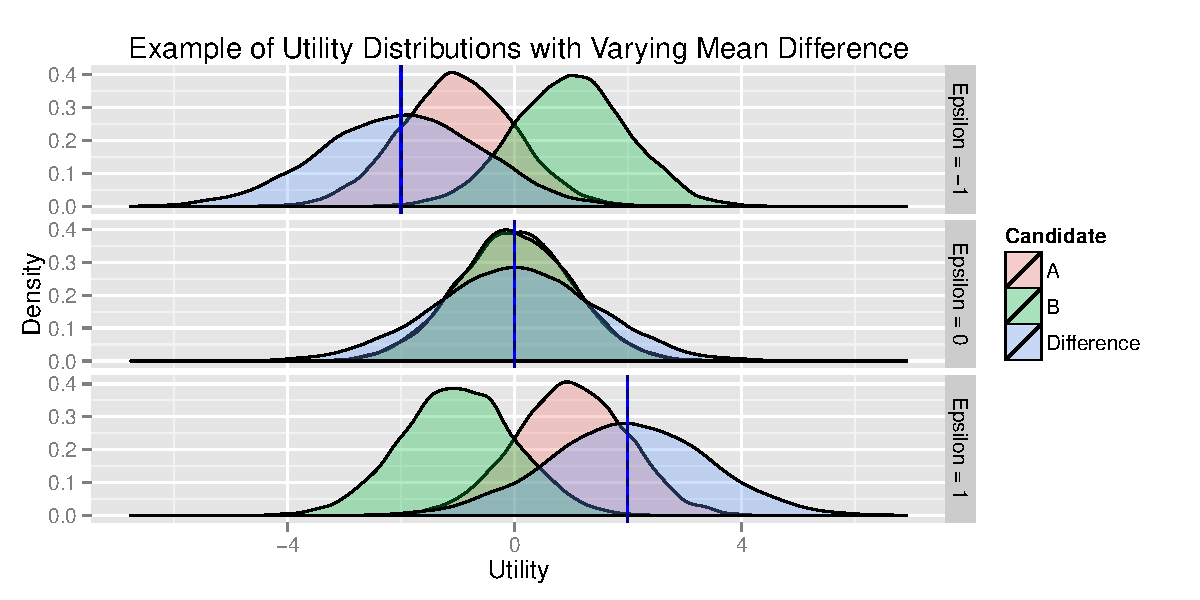
\includegraphics[width=\maxwidth]{figure/unnamed-chunk-2} 

\end{knitrout}


\clearpage
\subsubsection*{Scenario 1b: Independent Normal Utilities for two Alternatives}

\begin{align*}
U_a,U_b \sim \mathcal{N}(\mu=0,\sigma^2=1)
\end{align*}

\begin{knitrout}
\definecolor{shadecolor}{rgb}{0.969, 0.969, 0.969}\color{fgcolor}
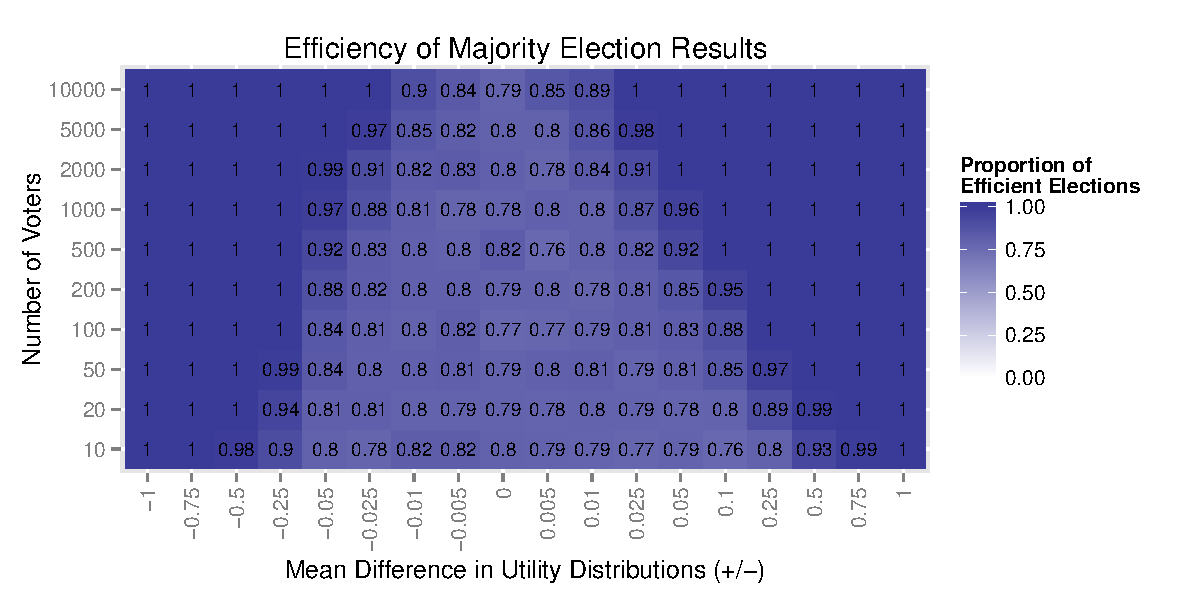
\includegraphics[width=\maxwidth]{figure/unnamed-chunk-3} 

\end{knitrout}


\clearpage
\subsubsection*{Scenario 2a: Utilities Determined by Uniform Ideal Points: Absolute Distance}

\begin{align*}
X_a,X_b,X_{cand1},X_{cand2} &\sim \mathcal{U}(0,1) \\
U_{a1,a2,b1,b2} &= -|X_{cand1,cand2}-X_{a,b}|
\end{align*}

\begin{knitrout}
\definecolor{shadecolor}{rgb}{0.969, 0.969, 0.969}\color{fgcolor}
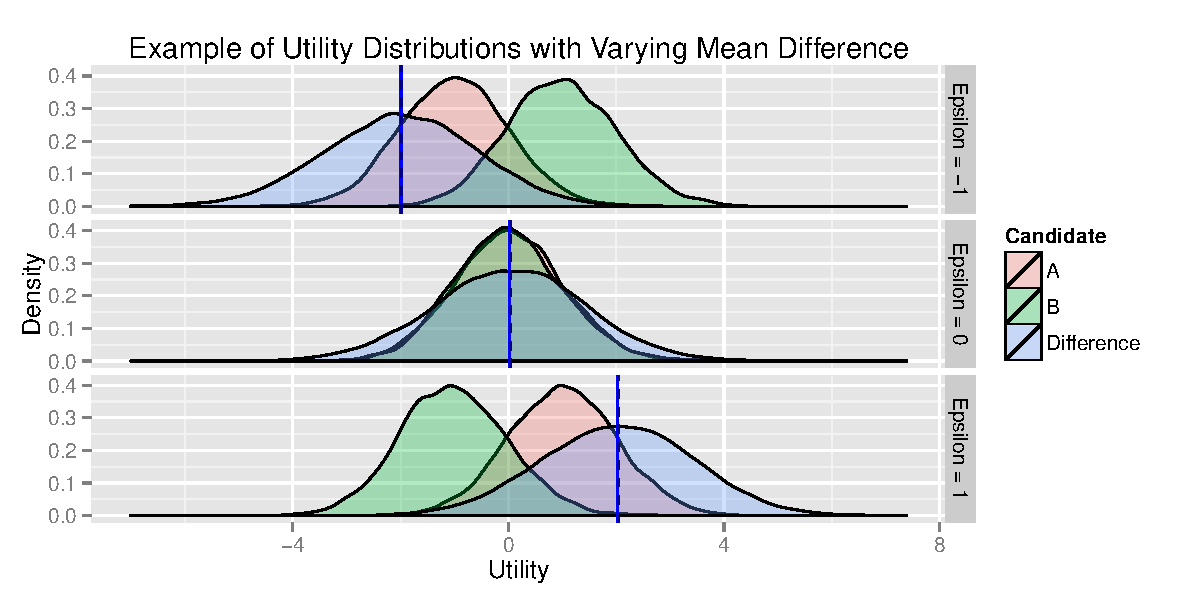
\includegraphics[width=\maxwidth]{figure/unnamed-chunk-4} 

\end{knitrout}


This is interesting: the bimodal differential is due to the fact that with absolute distances, the differential is equal for all individuals which are to the left or to the right of both available candidates. Accordingly, they all have the same utility differential, independent of their distance to either candidate.

\clearpage
\subsubsection*{Scenario 2b: Utilities Determined by Uniform Ideal Points: Squared Distance}

\begin{align*}
X_a,X_b,X_{cand1},X_{cand2} &\sim \mathcal{U}(0,1) \\
U_{a1,a2,b1,b2} &= -(X_{cand1,cand2}-X_{a,b})^2
\end{align*}

\begin{knitrout}
\definecolor{shadecolor}{rgb}{0.969, 0.969, 0.969}\color{fgcolor}
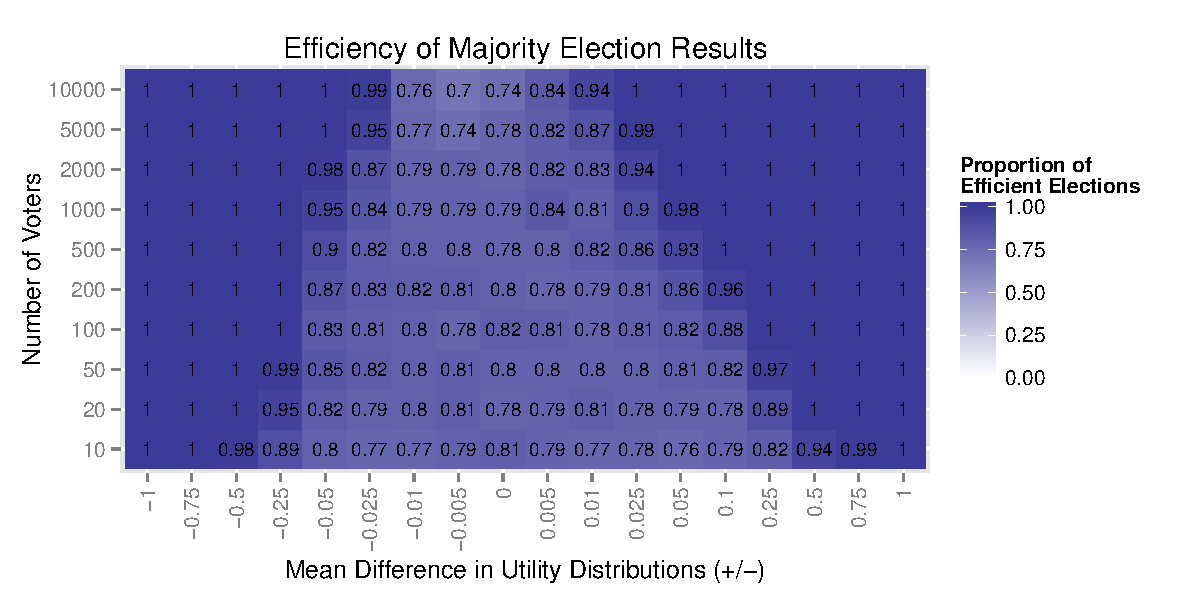
\includegraphics[width=\maxwidth]{figure/unnamed-chunk-5} 

\end{knitrout}


This is not the case if we look at squared distances rather than absolute distances (which is ususally the norm in most political science conceptualizations).

\clearpage
\subsubsection*{Scenario 3a: Utilities Determined by Normal Ideal Points: Absolute Distance}
\begin{align*}
X_a,X_b,X_{cand1},X_{cand2} &\sim \mathcal{N}(\mu=0,\sigma^2=1) \\
U_{a1,a2,b1,b2} &= -|X_{cand1,cand2}-X_{a,b}|
\end{align*}

\begin{knitrout}
\definecolor{shadecolor}{rgb}{0.969, 0.969, 0.969}\color{fgcolor}
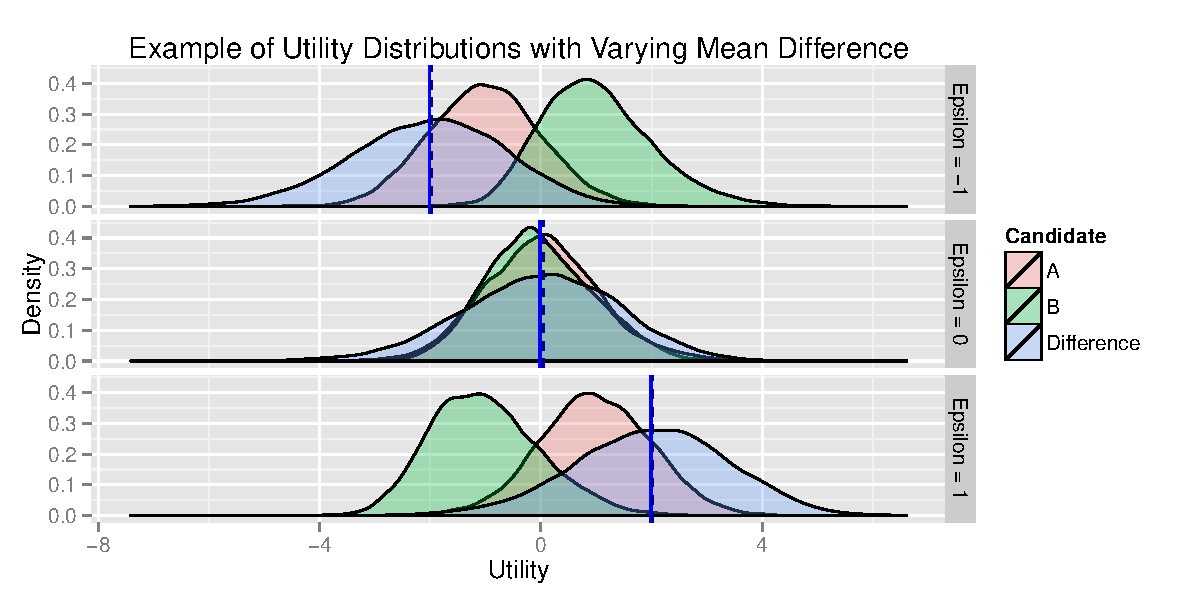
\includegraphics[width=\maxwidth]{figure/unnamed-chunk-6} 

\end{knitrout}


\clearpage
\subsubsection*{Scenario 3b: Utilities Determined by Normal Ideal Points: Squared Distance}
\begin{align*}
X_a,X_b,X_{cand1},X_{cand2} &\sim \mathcal{N}(\mu=0,\sigma^2=1) \\
U_{a1,a2,b1,b2} &= -(X_{cand1,cand2}-X_{a,b})^2
\end{align*}

\begin{knitrout}
\definecolor{shadecolor}{rgb}{0.969, 0.969, 0.969}\color{fgcolor}
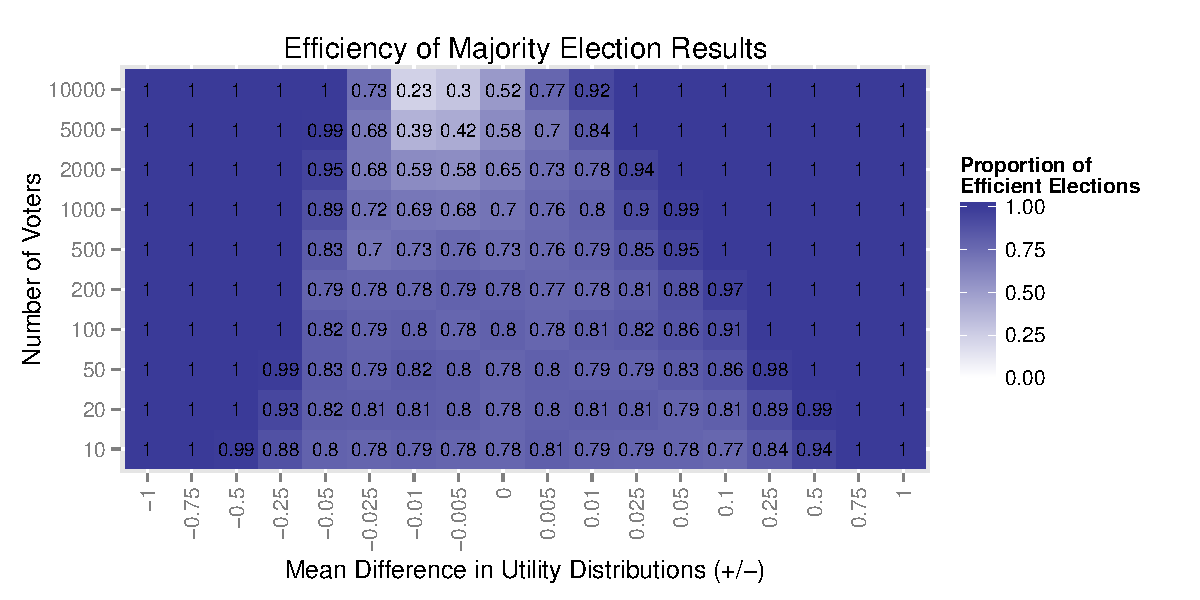
\includegraphics[width=\maxwidth]{figure/unnamed-chunk-7} 

\end{knitrout}


\clearpage
\subsubsection*{Scenario 4a: Positively Correlated Normal Utilities for two Alternatives}
\begin{align*}
U_a,U_b \sim \mathcal{N}\left(
\boldsymbol{\mu}=\begin{pmatrix}0 \\ 0\end{pmatrix},
\mathbf{\Sigma}=\begin{pmatrix}1 & 0.5 \\ 0.5 & 1\end{pmatrix}\right)
\end{align*}

\begin{knitrout}
\definecolor{shadecolor}{rgb}{0.969, 0.969, 0.969}\color{fgcolor}
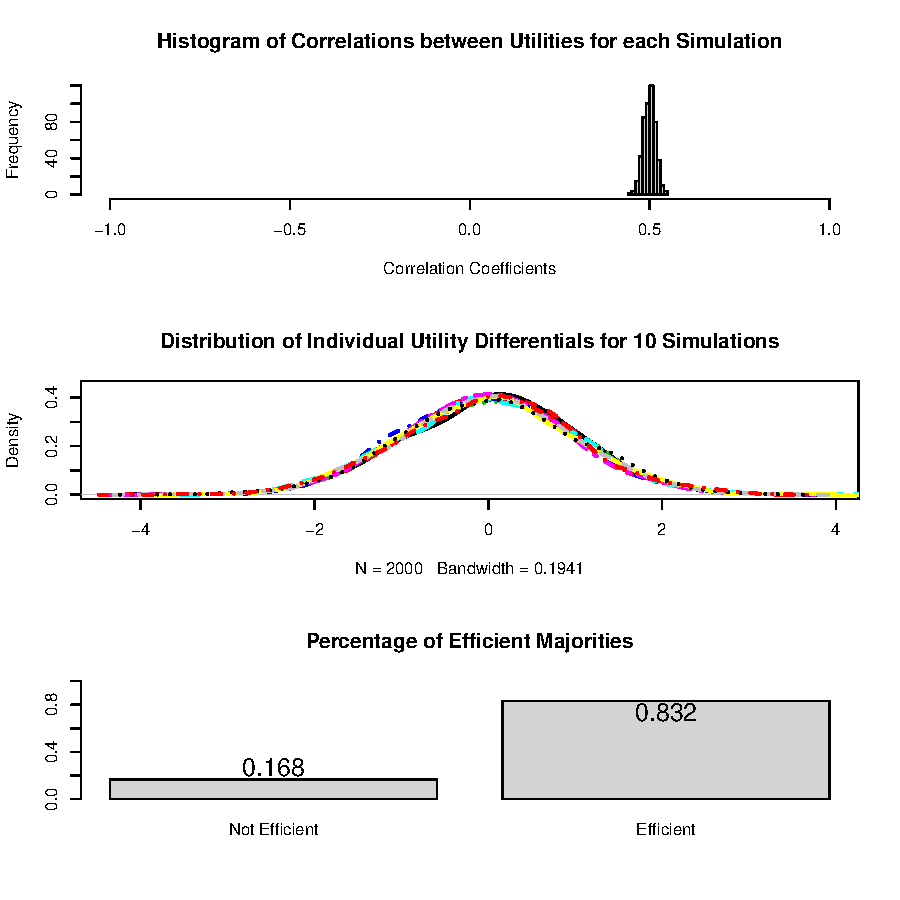
\includegraphics[width=\maxwidth]{figure/unnamed-chunk-81} 

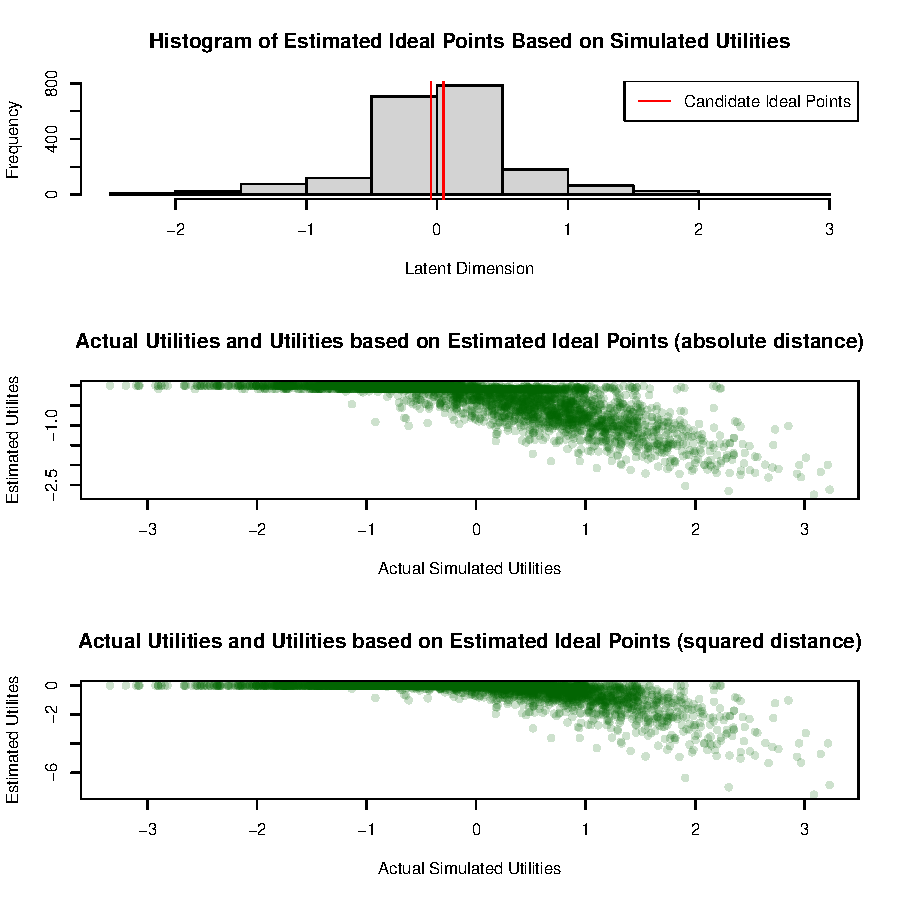
\includegraphics[width=\maxwidth]{figure/unnamed-chunk-82} 

\end{knitrout}


\clearpage
\subsubsection*{Scenario 4b: Negatively Correlated Normal Utilities for two Alternatives}
\begin{align*}
U_a,U_b \sim \mathcal{N}\left(
\boldsymbol{\mu}=\begin{pmatrix}0 \\ 0\end{pmatrix},
\mathbf{\Sigma}=\begin{pmatrix}1 & -0.9 \\ -0.9 & 1\end{pmatrix}\right)
\end{align*}

\begin{knitrout}
\definecolor{shadecolor}{rgb}{0.969, 0.969, 0.969}\color{fgcolor}
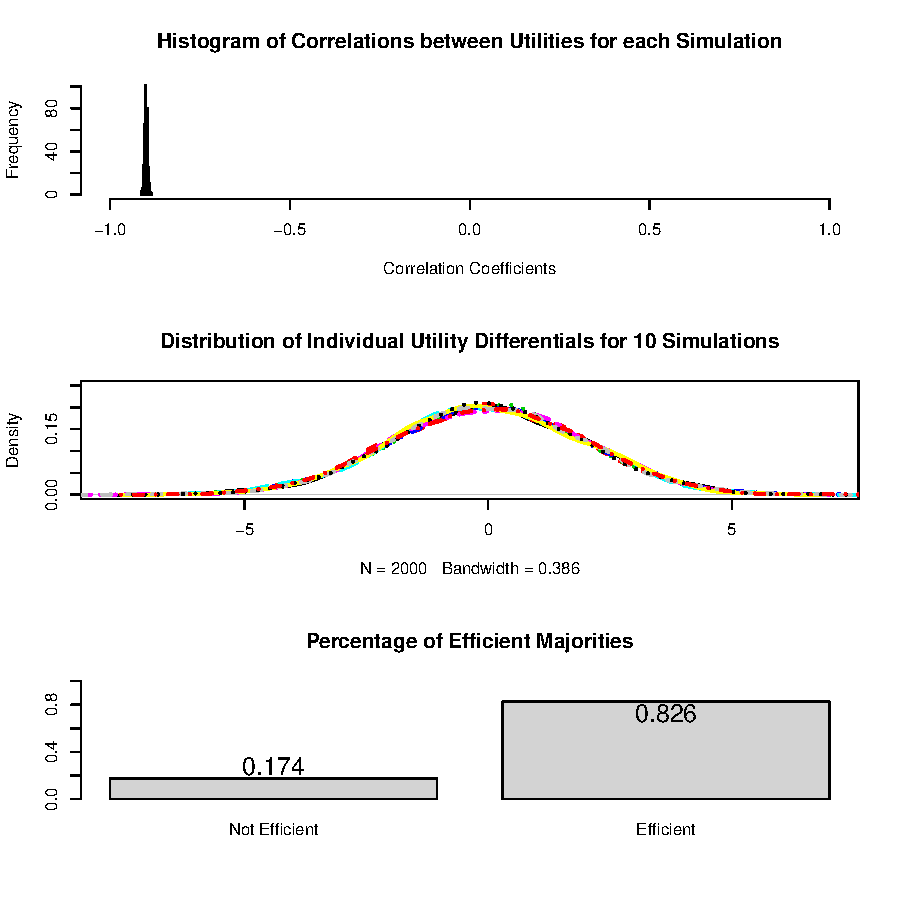
\includegraphics[width=\maxwidth]{figure/unnamed-chunk-91} 

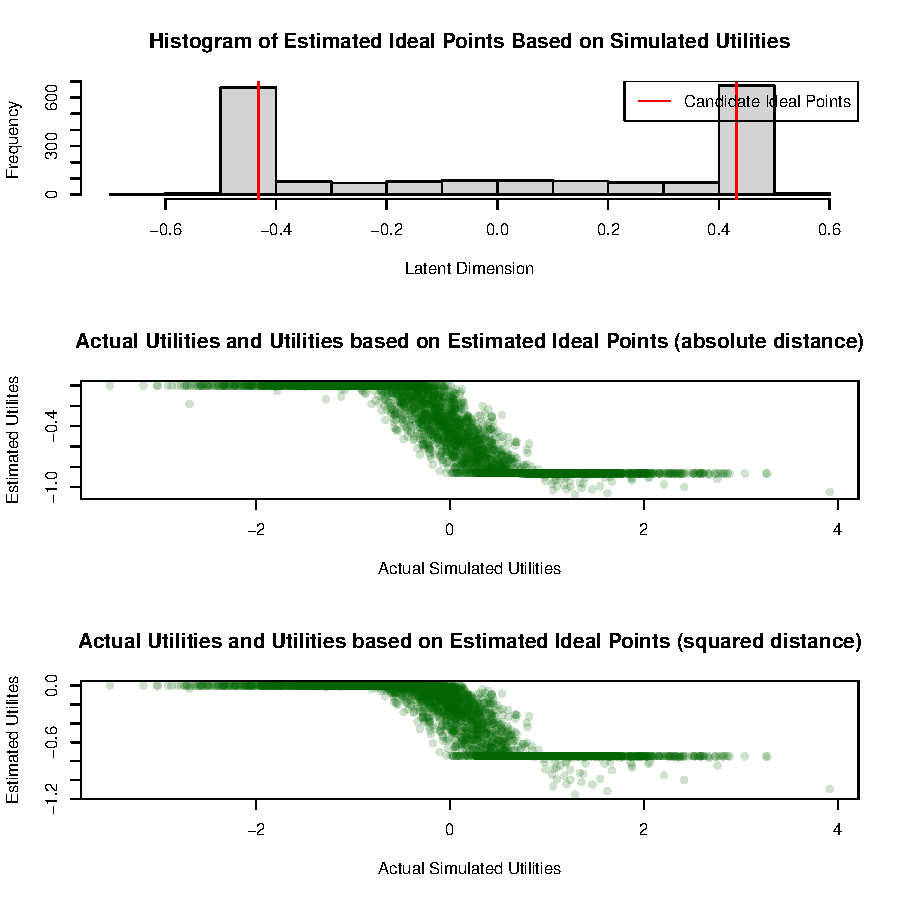
\includegraphics[width=\maxwidth]{figure/unnamed-chunk-92} 

\end{knitrout}


\clearpage
\subsection*{Second Set of Simulational Scenarios}
\subsubsection*{Scenario 5: Negatively or Positively Correlated Normal Utilities for two Alternatives}
In this scenario, I simulate two types of voters: one where the utilities are strongly negatively correlated and one type where they are moderately positively correlated. Each individual $i$ has a probability of $p=.5$ to be drawn from the following distribution:
\begin{align*}
U_a,U_b \sim \mathcal{N}\left(
\boldsymbol{\mu}=\begin{pmatrix}0 \\ 0\end{pmatrix},
\mathbf{\Sigma}=\begin{pmatrix}1 & -0.99 \\ -0.99 & 1\end{pmatrix}\right)
\end{align*}
as well as a probability of $1-p=.5$, to be drawn from the alternative distribution:
\begin{align*}
U_a,U_b \sim \mathcal{N}\left(
\boldsymbol{\mu}=\begin{pmatrix}0 \\ 0\end{pmatrix},
\mathbf{\Sigma}=\begin{pmatrix}1 & .5 \\ .5 & 1\end{pmatrix}\right)
\end{align*}

\begin{knitrout}
\definecolor{shadecolor}{rgb}{0.969, 0.969, 0.969}\color{fgcolor}
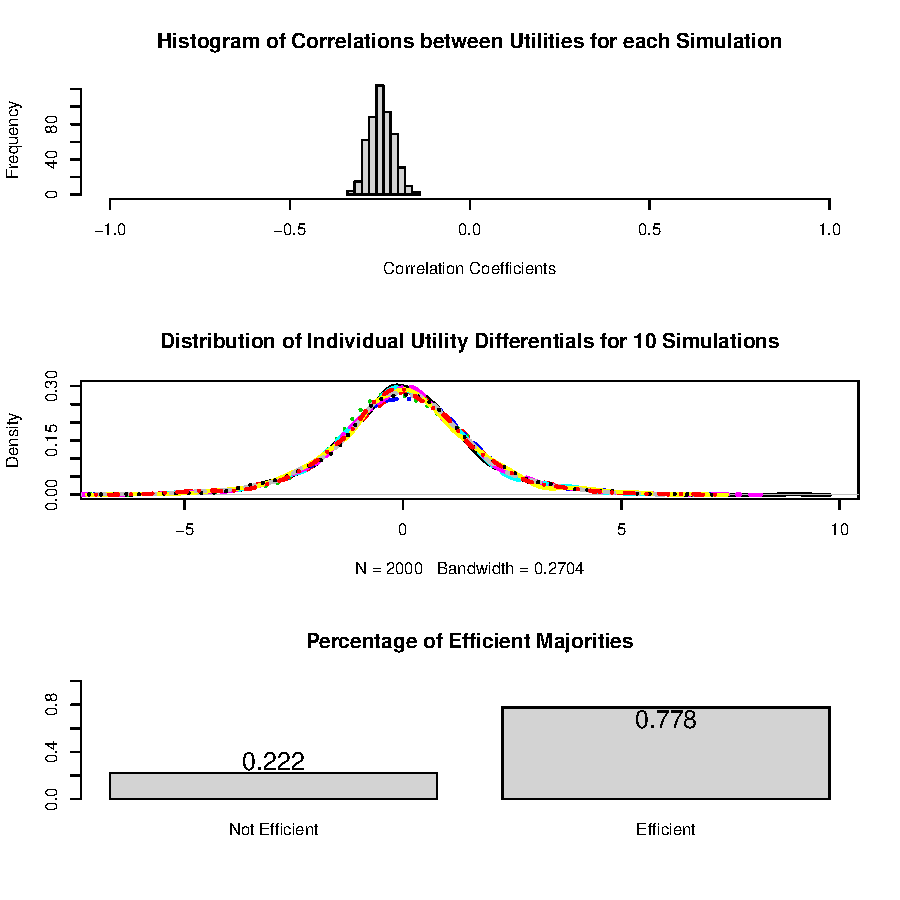
\includegraphics[width=\maxwidth]{figure/unnamed-chunk-101} 

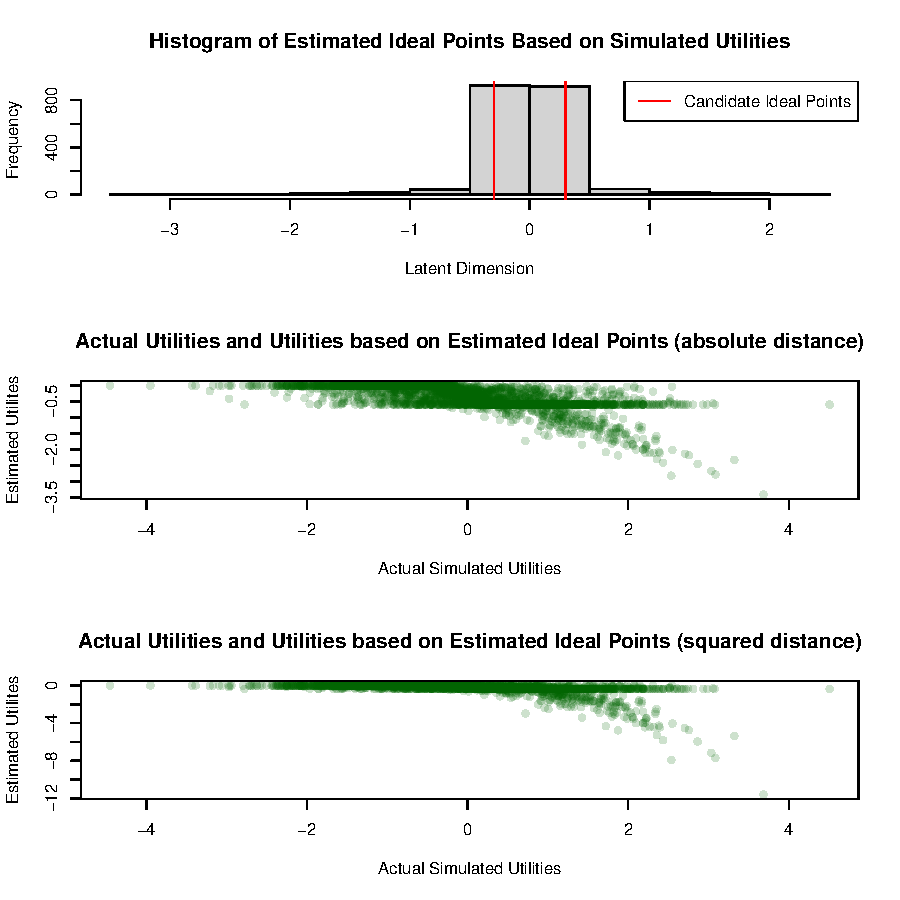
\includegraphics[width=\maxwidth]{figure/unnamed-chunk-102} 

\end{knitrout}


\clearpage
\subsubsection*{Scenario 6a: Normal Ideal Points/Squared Distance: Large Distance b/w Candidates}
\begin{align*}
X_a,X_b &\sim \mathcal{N}(\mu=0,\sigma^2=1) \\
X_{cand1} &\sim \mathcal{N}(\mu=1,\sigma^2=0.1) \\
X_{cand2} &\sim \mathcal{N}(\mu=-1,\sigma^2=0.1) \\
U_{a1,a2,b1,b2} &= -(X_{cand1,cand2}-X_{a,b})^2
\end{align*}

\begin{knitrout}
\definecolor{shadecolor}{rgb}{0.969, 0.969, 0.969}\color{fgcolor}
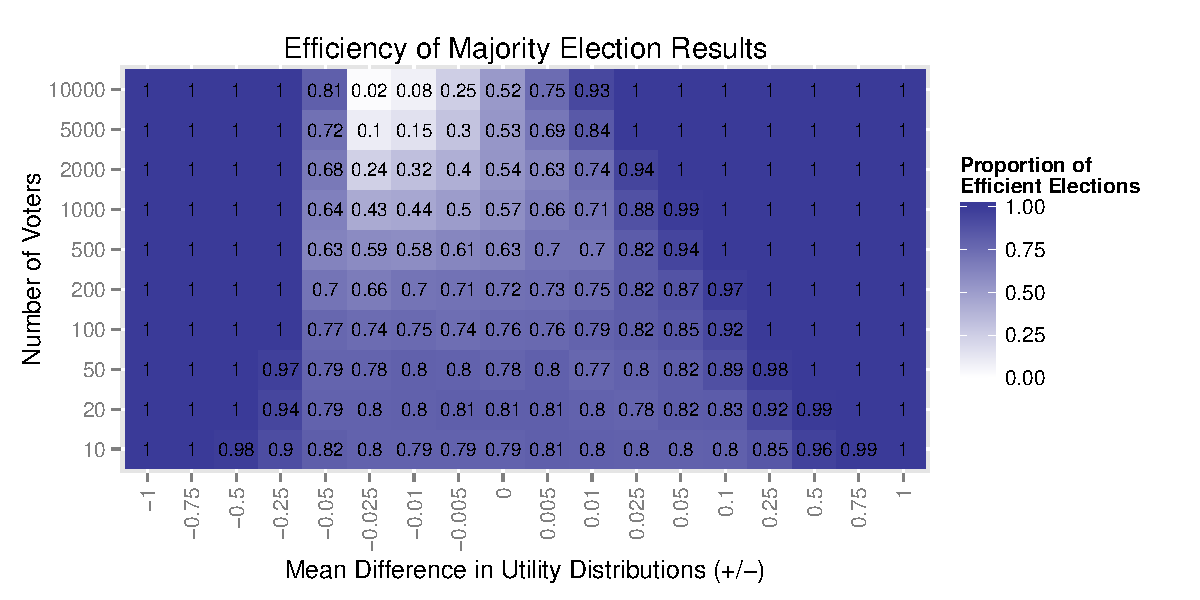
\includegraphics[width=\maxwidth]{figure/unnamed-chunk-11} 

\end{knitrout}


\clearpage
\subsubsection*{Scenario 6b: Normal Ideal Points/Squared Distance: Small Distance b/w Candidates}
\begin{align*}
X_a,X_b &\sim \mathcal{N}(\mu=0,\sigma^2=1) \\
X_{cand1},X_{cand2} &\sim \mathcal{N}(\mu=0,\sigma^2=0.1) \\
U_{a1,a2,b1,b2} &= -(X_{cand1,cand2}-X_{a,b})^2
\end{align*}

\begin{knitrout}
\definecolor{shadecolor}{rgb}{0.969, 0.969, 0.969}\color{fgcolor}
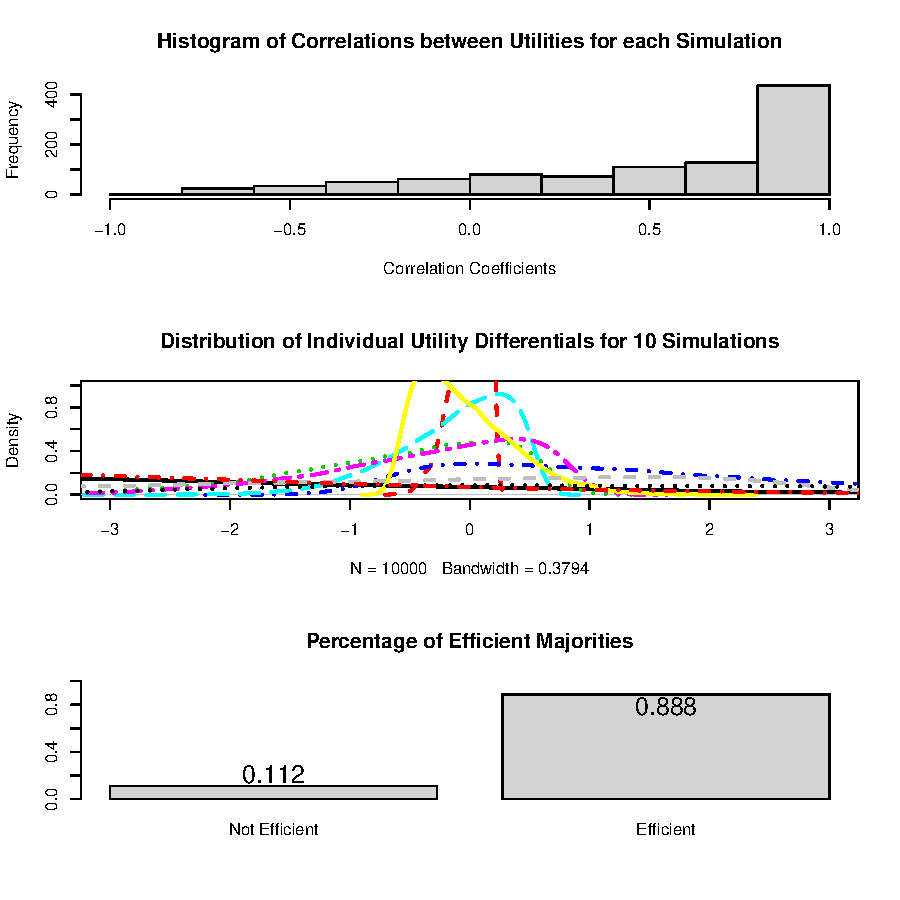
\includegraphics[width=\maxwidth]{figure/unnamed-chunk-12} 

\end{knitrout}


\clearpage
\subsubsection*{Scenario 7a: Utilities Determined by Skewed Ideal Points: Squared Distance}
\begin{align*}
X_a,X_b &\sim exp(\mathcal{N}(\mu=0,\sigma^2=10)) \\
X_{cand1},X_{cand2} &\sim \mathcal{N}(\mu=0,\sigma^2=0.1), \\
U_{a1,a2,b1,b2} &= -(X_{cand1,cand2}-X_{a,b})^2
\end{align*}

\begin{knitrout}
\definecolor{shadecolor}{rgb}{0.969, 0.969, 0.969}\color{fgcolor}
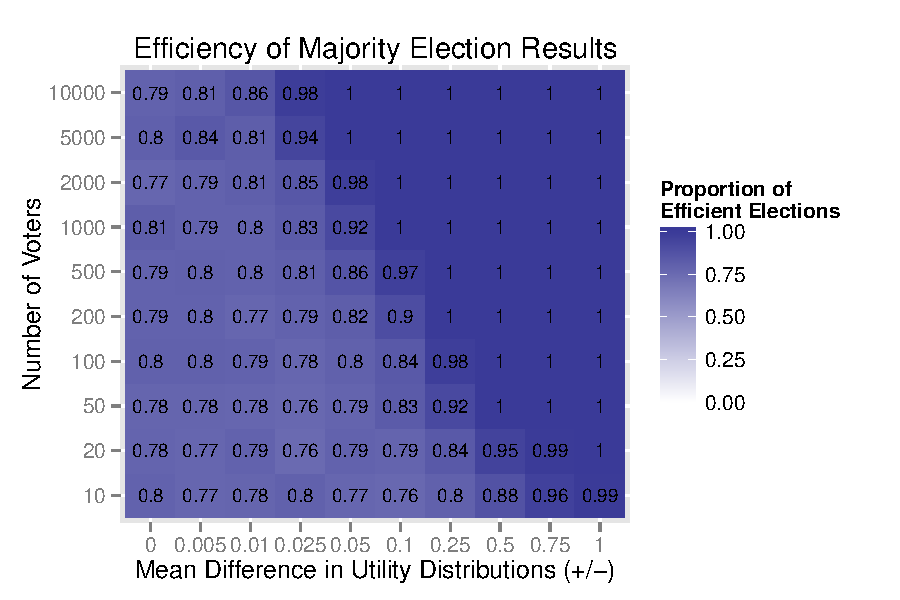
\includegraphics[width=\maxwidth]{figure/unnamed-chunk-13} 

\end{knitrout}


\clearpage
\subsubsection*{Scenario 7b: Utilities Determined by Skewed Ideal Points: Squared Distance}
\begin{align*}
X_a,X_b &\sim exp(\mathcal{N}(\mu=0,\sigma^2=10)) \\
X_{cand1},X_{cand2} &\sim \mathcal{U}(0,0.1), \\
U_{a1,a2,b1,b2} &= -(X_{cand1,cand2}-X_{a,b})^2
\end{align*}

\begin{knitrout}
\definecolor{shadecolor}{rgb}{0.969, 0.969, 0.969}\color{fgcolor}
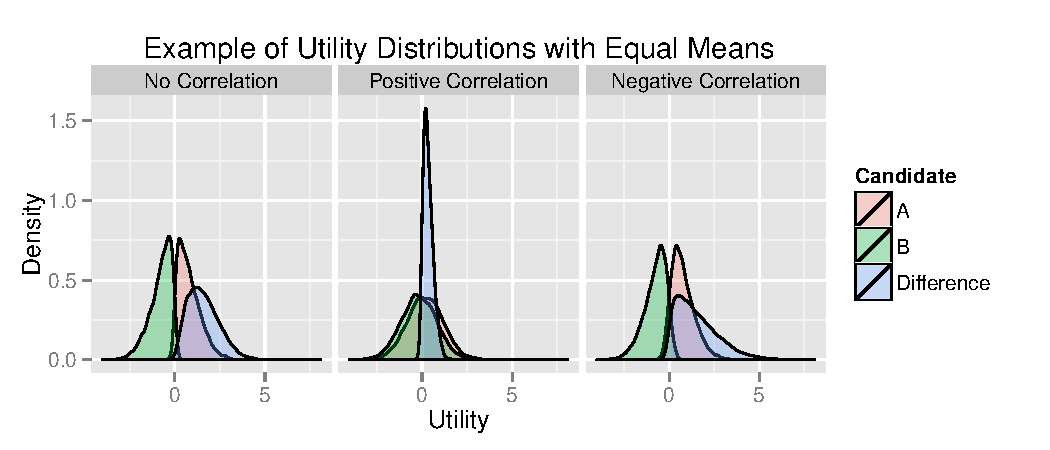
\includegraphics[width=\maxwidth]{figure/unnamed-chunk-14} 

\end{knitrout}


\clearpage
\subsubsection*{Scenario 8a: Different Independent Normal Utilities for two Alternatives: Large Distance}

\begin{align*}
U_a \sim \mathcal{N}(\mu=1,\sigma^2=0.1)\\
U_b \sim \mathcal{N}(\mu=-1,\sigma^2=0.1)
\end{align*}

\begin{knitrout}
\definecolor{shadecolor}{rgb}{0.969, 0.969, 0.969}\color{fgcolor}
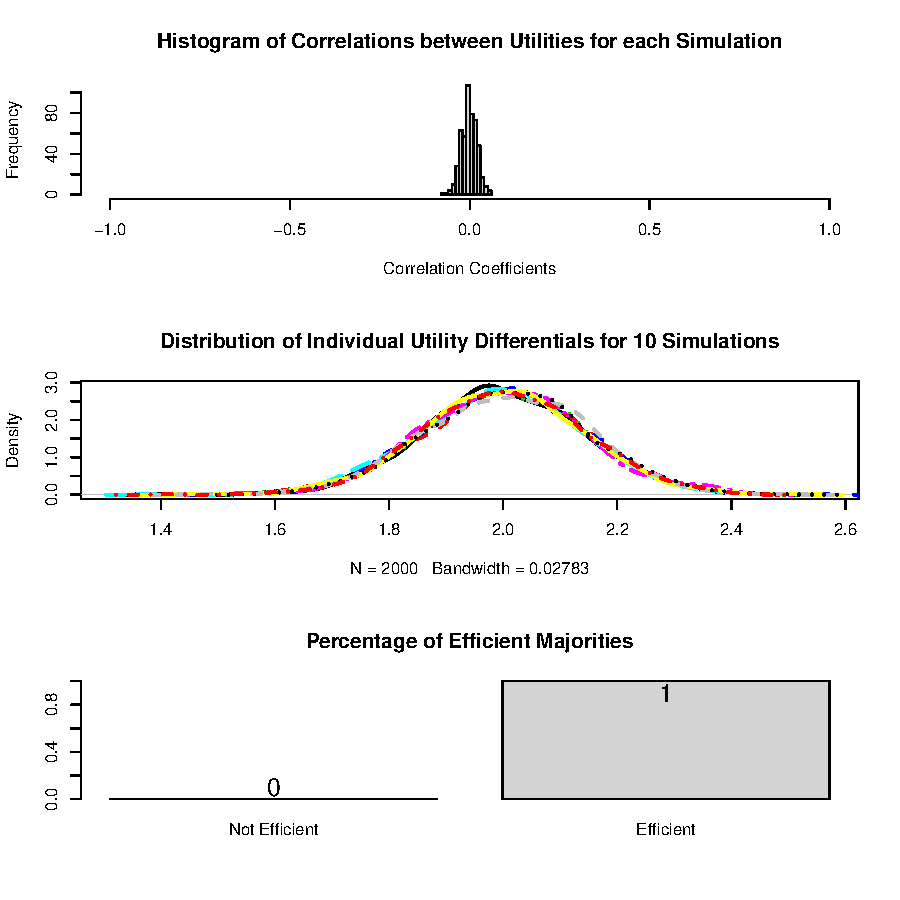
\includegraphics[width=\maxwidth]{figure/unnamed-chunk-151} 

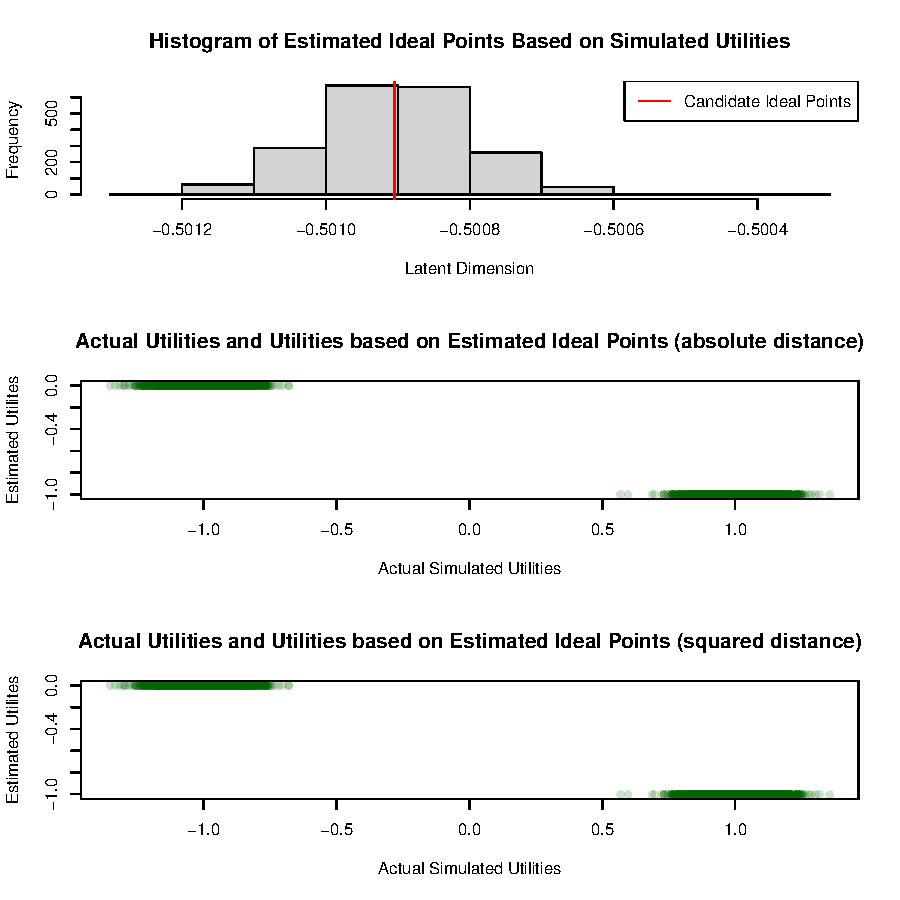
\includegraphics[width=\maxwidth]{figure/unnamed-chunk-152} 

\end{knitrout}


\clearpage
\subsubsection*{Scenario 8b: Different Independent Normal Utilities for two Alternatives: Small Distance}

\begin{align*}
U_a \sim \mathcal{N}(\mu=0,\sigma^2=0.1)\\
U_b \sim \mathcal{N}(\mu=0,\sigma^2=0.1)
\end{align*}

\begin{knitrout}
\definecolor{shadecolor}{rgb}{0.969, 0.969, 0.969}\color{fgcolor}
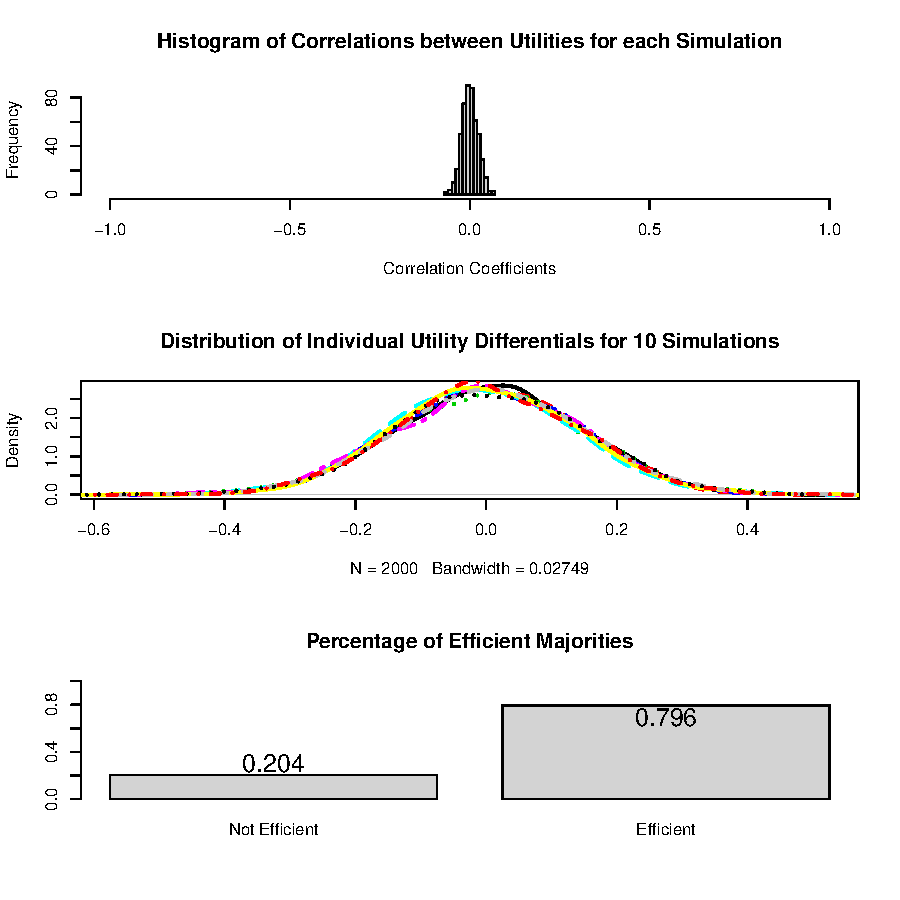
\includegraphics[width=\maxwidth]{figure/unnamed-chunk-161} 

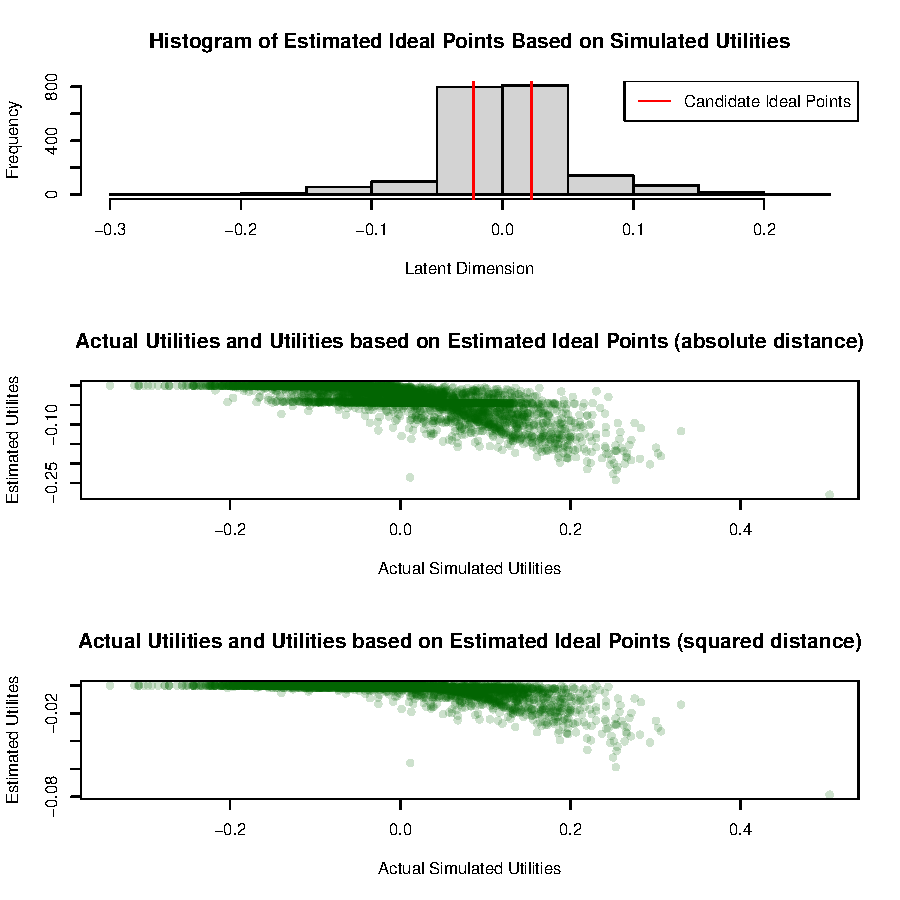
\includegraphics[width=\maxwidth]{figure/unnamed-chunk-162} 

\end{knitrout}


\clearpage
\subsubsection*{Scenario 8c: Different Independent Normal Utilities for two Alternatives: Heterogenous Population}
In this scenario, I simulate two types of voters: one where the utilities are very close and one type where they are further apart. Each individual $i$'s utilities have a probability of $p=.5$ to be drawn from the following distribution:
\begin{align*}
U_a \sim \mathcal{N}(\mu=0,\sigma^2=0.1)\\
U_b \sim \mathcal{N}(\mu=0,\sigma^2=0.1)
\end{align*}
as well as a probability of $1-p=.5$, to be drawn from the alternative distribution:
\begin{align*}
U_a \sim \mathcal{N}(\mu=1,\sigma^2=0.1)\\
U_b \sim \mathcal{N}(\mu=-1,\sigma^2=0.1)
\end{align*}

\begin{knitrout}
\definecolor{shadecolor}{rgb}{0.969, 0.969, 0.969}\color{fgcolor}
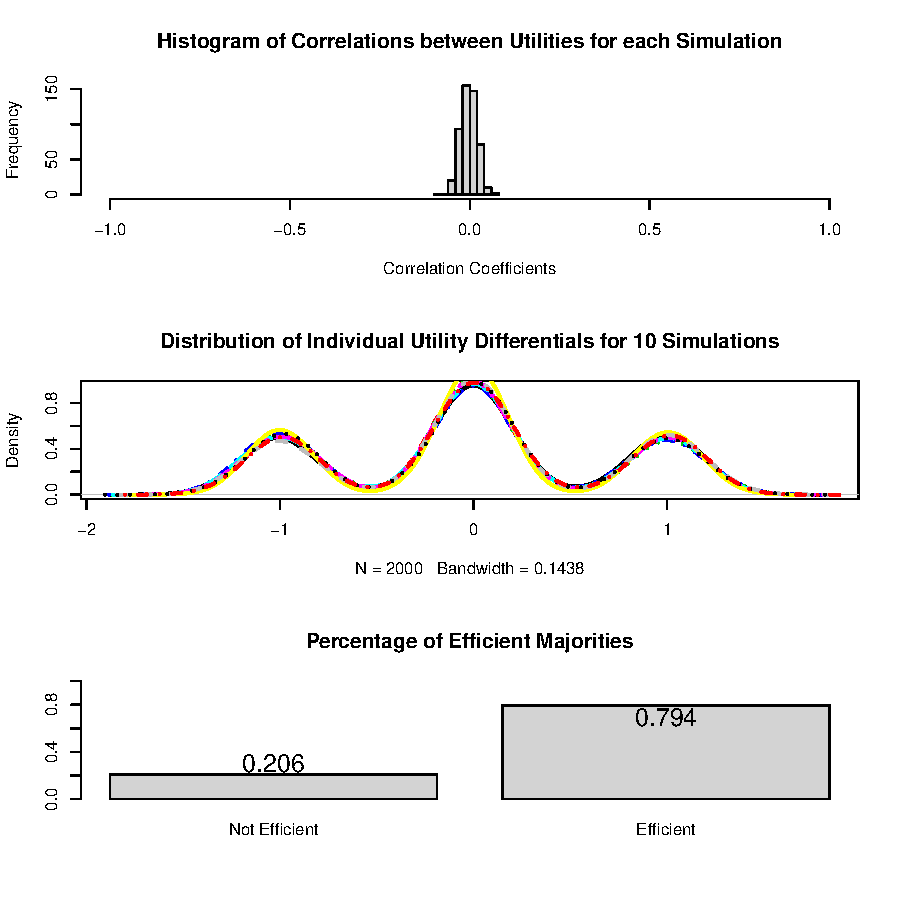
\includegraphics[width=\maxwidth]{figure/unnamed-chunk-171} 

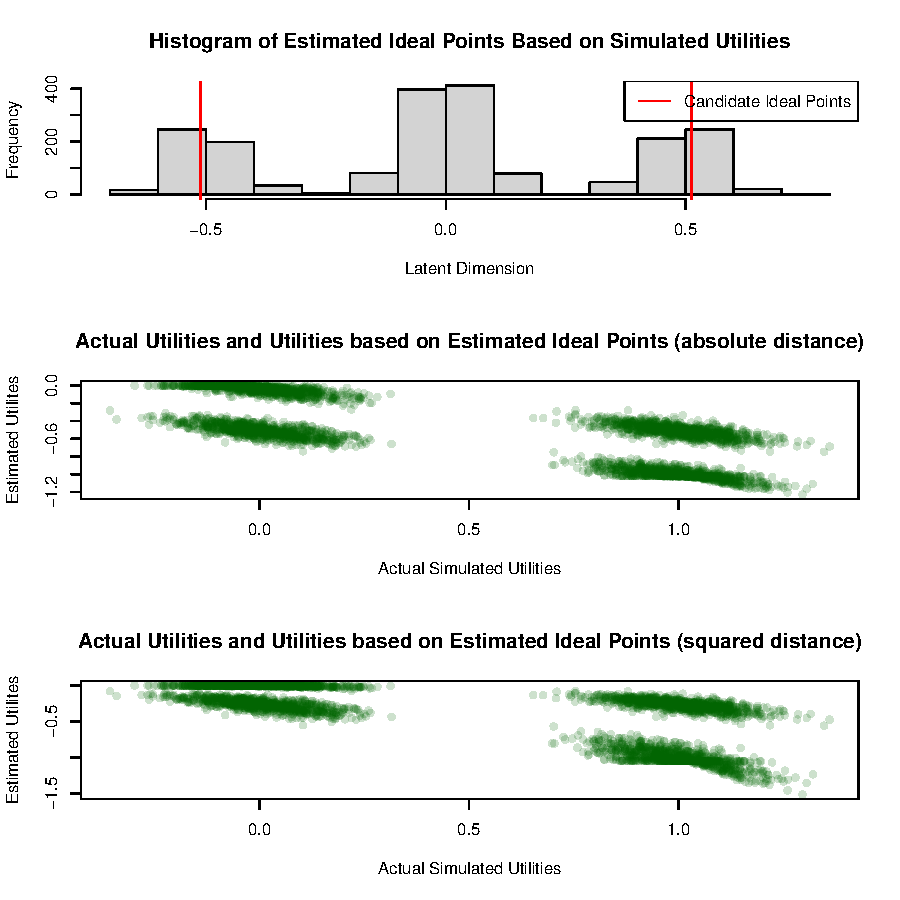
\includegraphics[width=\maxwidth]{figure/unnamed-chunk-172} 

\end{knitrout}


%\bibliographystyle{apsr}
%\bibliography{Literature}
\end{document}
